\documentclass[class=NCU_thesis, crop=false]{standalone}
\usepackage{braket}
\usepackage{mathtools}

\begin{document}

\chapter{實驗架設}
本章會先簡單介紹實驗上會用到的關鍵儀器,說明其特性與相關設定,並描述元件使用的優化方式與可能造成誤差之原因。再來會介紹兩種光源的製備,說明光源的特性、產生機制、調變方式與測量方法。

\section{偽隨機訊號產生器}
由於實驗上無法產生真正的隨機訊號,只能使用偽隨機訊號產生器 (Pseudo Random Bit Sequence, PRBS),儀器型號為 MP1763C (Anritsu),可以產生 0.5 至 12.5 Gb/s 的偽隨機訊號,裝置如\cref{fig:PRBS_machine}。偽隨機訊號實際上為週期訊號,會重複出現特定的隨機序列,其週期可以調整,為了達到最接近隨機的效果,我們選擇使用最長的隨機序列,一個週期內共有 $2^{31}-1$ 的隨機位元。

我們實驗上實際使用的偽隨機訊號產生率 10 Gb/s,每秒能產生 $10\times 10^{9}$ 個隨機位元,以示波器(Infiniium DCA-J 86100C, Agilent,使用的模組為 86112A, Agilent)去測量該訊號的眼圖 (eye diagram) ,眼圖是一種用來檢測訊號品質之測量示波器顯示模式,會以資料速度(data rate)作為觸發水平更新,將特定時間內的測量結果重疊於畫面中,並計算訊號的上升與下降時間(rising and falling time)、抖動(jitter)、交叉振幅(crossing)\dots 等資訊,量測結果如\cref{fig:prbs_eye},可見實際訊號與理論\cref{fig:PRBS_simulation} 有很大的差異,實際的訊號會有不小的上升與下降時間,圖形的上下也不太對稱,這都會影響到展頻與壓縮的效果,造成實驗與理論的誤差。

\fig[0.5][fig:PRBS_machine][!htb]{PRBS_machine.jpg}[高頻偽隨機訊號產生器裝置圖]


\begin{figure}[!hbt]
    %\captionsetup[subfigure]{labelformat=empty} % 完全隱藏圖號
    \centering
    \subcaptionbox
        {輸入第一台 EOM 之隨機訊號
        \label{fig:subfig_fig1}}
        {\includegraphics[width=0.4\linewidth]{data.bmp}}
    ~~~~
    \subcaptionbox
        {輸入第二台 EOM 之隨機訊號
        \label{fig:subfig_fig2}}
        {\includegraphics[width=0.4\linewidth]{data_bar.bmp}}
    \caption{PRBS 輸出之訊號眼圖(放大前)}
    \label{fig:prbs_eye}
\end{figure}

\section{電光調製器}

電光調製器 (Electro-Optic Modulator, EOM) 可使用電訊號對光進行調製,一般而言可以分成三種,分別為振幅、相位與偏振的調製,在我們的實驗中需要調製的是相位。使用的儀器為 EOSPACE 的 SN73717 與 SN73718,分別為頻譜的展寬與壓縮用,裝置如\cref{fig:eom}。

\fig[0.7][fig:eom][!htb]{eom_machine.png}[我們分別將兩台 EOM 置於盒中提供保護,並以塔狀堆疊節省光路空間。][實驗使用之兩台電光調製器]

相位調制器由鈮酸鋰 ($LiNbO_{3}$) 雙折射晶體製成,因泡克耳斯效應 (Pockels effect),外加電場能線性的改變作用方向上之晶體折射率,進而達到改變相位的效果,我們定義能入射光相位改變 $\pi$ 之電訊號電壓為 $V_{\pi}$。

由上介紹可知,實際使用上需優化進光的偏振以及電訊號的振幅,以達到預期的相位調製效果。所以我們會在 EOM 前放置一個偏極片(Polarizer)半波片 (half-wave plate) ,如\cref{fig:eom_setup},藉由調整兩者的角度,使光能以最佳的線偏角度入射 EOM。

\fig[0.75][fig:eom_setup][!htb]{eom_setup.png}[EOM 及相關元件架設。使用上我們會先讓光通過一偏極片,確定光為線偏振,再以半波片旋轉偏振的角度,優化調製之效果。][EOM 及相關元件架設]

\section{高頻電訊號放大器}

由於我們使用的隨機訊號產生器僅能輸出 0.2 至 2 $V_{pp}$ 的訊號,而 EOM 的 $V_{\pi}$ 高於 2 V,所以需再經過放大器才能提供足夠的電壓去進行相位調製。

我們使用的放大器型號為 OA3MVM (Centallax),輸入的訊號會經過三階段的放大,每一階段各需要兩個電壓去驅動,分別為 $V_{g}$ 與 $V_{d}$,這組電壓的大小會影響放大的大小與速度,因此我們做了一個穩壓電路,能一次輸出 3 個 $V_{g}$ 與 3 個 $V_{d}$,裝置如\cref{fig:amp_circuit}。

\fig[0.75][fig:amp_circuit][!htb]{amp_circuit.png}[放大器與穩壓電路]

同樣的,也用示波器去測量眼圖,架設如\cref{fig:amplifier_setup},觀察經放大後的訊號品質,如\cref{fig:amp_prbs_eye},可明顯看出訊號變得更不穩定,且兩台 EOM 使用的電訊號形狀也不同,這是由兩邊使用的連接線(SAM-to-SMA)的長度與材質均不同,會有不一樣的頻率響應與耗損,使兩個訊號無法互補,這會對頻譜壓縮與還原的效果造成負面的影響。

\fig[0.75][fig:amplifier_setup][!htb]{amplifier_setup.png}[將隨機訊號經過放大器並以示波器測量眼圖之電路架設]

\begin{figure}[!hbt]
    %\captionsetup[subfigure]{labelformat=empty} % 完全隱藏圖號
    \centering
    \subcaptionbox
        {輸入第一台 EOM 之隨機訊號
        \label{fig:subfig_fig1}}
        {\includegraphics[width=0.4\linewidth]{amp_data.bmp}}
    ~~~~
    \subcaptionbox
        {輸入第二台 EOM 之隨機訊號
        \label{fig:subfig_fig2}}
        {\includegraphics[width=0.4\linewidth]{amp_data_bar.bmp}}
    \caption{PRBS 輸出之訊號眼圖(放大後)}
    \label{fig:amp_prbs_eye}
\end{figure}

我們可從眼圖的測量結果去量化訊號品質,放大前後的比較如\cref{tab:amplifier_compare},從圖和表中能觀察到,輸入第二台 EOM 用的訊號在放大後變得很不穩定,這是因為那端使用的電線長度很長(長邊約 400 公分,短邊約 80 公分),且那條線材已經放了十年,傳輸品質會下降,會有較大的損耗以及較明顯的色散現象,使訊號失真,這會降低我們頻譜壓縮的效果。

\begin{table}[h]
    \centering
    \caption{訊號失真與不穩定之量化指標}
    \begin{tabular}{| c | c | c | c |}
\hline
         & jitter & amplitidu & rising \& falling
    \\ \hline
    \multicolumn{4}{|c|}{輸入第一台 EOM 用之隨機訊號}\\ \hline
    放大前 & 10 ps & $\pm$5.8\% & 38 ps\\ \hline
    放大後 & 14 ps & $\pm$7.7\% & 38 ps\\ \hline
    \multicolumn{4}{|c|}{輸入第二台 EOM 用之隨機訊號}\\ \hline
    放大前 & 9 ps & $\pm$6.5\% & 35 ps\\ \hline
    放大後 & 17 ps & $\pm$16.7\% & 74 ps\\ \hline
    \end{tabular}
    \label{tab:amplifier_compare}
\end{table}

\section{電訊號相位延遲器}
如\cref{section:time_delay} 所述,想要對已展頻的光做反向的調製,必須精準的控制兩台 EOM 電訊號的時間差,所以我們會在其中一邊的電路加上一個相位延遲器,其型號為 Model 981(api technologies corp.),如\cref{fig:phase_shifter},可以藉由調整側邊拉桿的長度來微調電訊號的相位。根據其規格書上的標示,此相位延遲器最多能讓 1 GHz 的訊號延遲 60 度的相位,相當於 1.67 ns 的時間差。若電訊號的傳輸速度以三分之二光速來計算的話,此時間差等同於 3.33 公分的電路長度差。

\fig[0.45][fig:phase_shifter][!htb]{phase_shifter.png}[電訊號相位延遲器]

\section{光源製備}

\subsection{雷射光}
雷射光源為 TOPTICA 的 DLC TA-SHG PRO 雷射系統,可產生中心波長約為 795 nm 的窄頻雷射。此雷射的特點為出光頻率可調,可以透過電壓大小來改變共振腔上光柵的角度,以調整出光的頻率,實際上會用電腦控制,經由資料擷取器(DAQ, Data Acquisition Device)輸出電壓至雷射系統。此外,我們還會將光源一分為二,將其中一道光做為參考光(reference light)打入波長計(wavemeter),其型號為 WSU 30(HighFinesse),可由電腦讀出雷射的頻率與波長等數值。結合前述的電壓控制與波長讀值,可形成一個 PID(proportional–integral–derivative)回饋系統,我們能以此系統精準的調整雷射頻率,將其穩定度控制在 2 MHz 內。

除了波長 795 nm 的紅光外,雷射系統內還有一塊置於共振腔內的非線性晶體,可將前述的紅光打入內,以倍頻效應 (Simple-Harmonic Gemeration, SHG) 產生波長為 397.5 nm 的藍光,可用來打入另一塊非線性晶體,以自發參量下轉換 (Spontaneous Parametric Down-Conversion, SPDC) 的過程產生 795 nm 的雙光子。

\subsection{單光子}
\label{subsection:single_photon}
雙光子的產生機制為 SPDC,入射一道波長 397.5 nm 的藍光雷射進入 PPKTP (Periodically Poled KTP)晶體,產生 Type-II 的時間 - 能量糾纏光子對 (time-energy entangled biphoton),波長約為 795 nm,產生出來的光須滿足能量守恆與動量守恆,如\cref{eq:quasi_phase_matching} ,我們稱其為準相位匹配條件 (quasi phase matching condition) ,其中 $\vec{k_m}$ 為晶體週期性極化反轉提供之動量補償項。

\begin{equation}
\begin{split}
    \omega_p &=\omega_s+\omega_i\\
    \vec{k_p} &=\vec{k_s}+\vec{k_i}+\vec{k_m}
\label{eq:quasi_phase_matching}  
\end{split}
\end{equation}
    

在晶體設計中,我們會在晶體的末端鍍上 397.5 nm 的高反射薄膜,使入射藍光在末端被反射,此舉等效於將晶體變為兩倍長,從\cref{fig:gain_curve} 的增益曲線(gain curve)中可知,當晶體長度 L 變兩倍,增益曲線會變窄\cite{chuu2012miniature}。除此之外,還會在晶體兩端都度上 795nm 的高反射薄膜,使晶體本身形成一個紅光的共振腔,只有在增益曲線內且符合能量守恆的共振模態才會產生雙光子對。基於上述的兩種鍍膜帶來的效果,這樣的設計能讓我們產生出接近單模(single mode)的窄頻光子\cite{wu2017bright},且相對的會有較長的相干時間 (coherence time) ,利於我們對光子的時間波包進行調製。

\fig[0.75][fig:gain_curve][!htb]{gain_curve.png}[雙光子產生機制,下半部為晶體之增益曲線;上半部為共振模態,$\omega_s$ 與 $\omega_i$ 互相重疊的部分為符合能量守恆條件的模態。僅有在增益曲線內且符合能量守恆的模態會被產生。][雙光子產生機制]

實驗上會將產生出來的雙光子對經過 PBS (polarization beam splitter),將訊號分為 signal 和 idler,以 idler 做為觸發訊號,先對 idler 進行測量,這時另一顆光子 signal 被稱為前驅單光子(heralded single photon),此為我們實驗使用之單光子源,會再讓其經過 $^{87}Rb$ 原子氣體管與 EOM,讓光子被吸收或對其進行相位的調製,並做 $G^{2}(\tau)$\cite{PhysRevLett.101.103601} 的測量,$G^{2}(\tau)$ 的定義如 (\ref{eq:g2_definition_original})。

\begin{equation}
\begin{split}
    G^{2}(\tau)&=\braket{a^{\dagger}_{i}(t+\tau)a^{\dagger}_{s}(t)a_{s}(t)a_{i}(t+\tau)}\\
    &=R^2+\frac{4\Gamma_{s}\Gamma_{i}}{\Gamma_{s}+\Gamma_{i}}\left\{\begin{matrix}
        e^{\Gamma_{s}\tau} & ,\tau<0\\
        e^{-\Gamma_{i}\tau} & ,\tau>0
        \end{matrix}\right.
\label{eq:g2_definition_original}
\end{split}
\end{equation}

此為二階強度關聯函數 (second-order intenstiy correlation function),$\tau$ 為兩顆單光子抵達探測器(SPCM-AQRH-14-FC, Excelitas Technologies)的時間差,\cref{eq:g2_definition_original} 中的 $R^2$ 項為不具時間關聯之單光子,在激發強度弱的時候它會遠小於雙光子的訊號,所以實驗上我們可以將\cref{eq:g2_definition_original} 簡化成 \cref{eq:g2_definition_original} 來分析。在符合準相位匹配條件時能最有效率的產生雙光子,實際測量結果如\cref{fig:single_photon_g2},此光子之時間波包寬度約為 50 ns,將波包雙邊的衰減時間$\Gamma_{s}$ 及 $\Gamma_{i}$ 帶入\cref{eq:bandwidth}\cite{chuu2012miniature},可計算出光子的頻寬約為 4.5 MHz。

\begin{equation}
    \begin{split}
        G^{2}(\tau)=\frac{4\Gamma_{s}\Gamma_{i}}{\Gamma_{s}+\Gamma_{i}}\left\{\begin{matrix}
            e^{\Gamma_{s}\tau} & ,\tau<0\\
            e^{-\Gamma_{i}\tau} & ,\tau>0
            \end{matrix}\right.
    \label{eq:g2_definition}
    \end{split}
\end{equation}

\begin{equation}
        \Delta \omega=[(\sqrt{\Gamma^4_s+6\Gamma^2_s \Gamma^2_i+\Gamma^4_i}-\Gamma^2_s-\Gamma^2_i)/2]^{1/2}
    \label{eq:bandwidth}
\end{equation}

\fig[0.75][fig:single_photon_g2][!htb]{nocell_spread_no_etalon.png}[糾纏光子對之 $G^{2}(\tau)$ 量測]

為了找到符合準項未匹配條件的入射光波長與晶體溫度,實驗上會以\cref{fig:temp_scanning_setup} 的光路架設,將入射紅光的頻率固定在 3771054890 MHz,改變 PPKTP 晶體溫度測量雙光子的產生率 (biphton rate),結果如\cref{fig:temp_scan_g2},在 39.91$^{\circ}C$ 至 40.10$^{\circ}C$ 有四組符合條件的模態,紅線與黑線分別為有放與沒放 $^{87}Rb$ 原子氣體管時之測量結果,兩者比較可以發現在第二和第三個的模態中雖有明顯的吸收,但吸收率不高,我們認為這是因為在頻域上晶體所產生的光子為多模 (multi-mode) 而非單模 (single-mode),同時產生了兩種以上頻率的單光子,儘管其中一個頻率的光子能完全被原子吸收,其他頻率的光子仍會透射,因此無法讓透射率趨近於零。

\fig[0.75][fig:temp_scanning_setup][!htb]{temp_scanning_setup.png}[固定入射光頻率,調整 PPKTP 晶體溫度測量雙光子的產生率]

\fig[0.75][fig:temp_scan_g2][!htb]{temp_scanning.png}[調整溫度測量雙光子產生率,黑線為直接對雙光子進行量測;紅線為先讓其中一顆單光子通過 $^{87}Rb$ 氣體管再測量,其中第二和第三個模態的穿透率下降,表示有部分的光被 $^{87}Rb$ 原子吸收。][調整溫度測量雙光子產生率]

以我們使用之晶體的長度與折射率估計,FSR 約為 5 GHz,所以兩個模態的頻率差一定大於 5 GHz,我們可在 $^{87}Rb$ 氣體管前面加上一個頻寬為 60 MHz 的 Etalon 濾波器(參見\cref{section:etalon}),只允許特定頻率附近的光通過,實驗架設如 \cref{fig:temp_scanning_setup_with_etalon},先不放 $^{87}Rb$ 原子氣體管時,比較有無 Etalon 濾波器時測量之結果,如\cref{fig:temp_scan_g2_with_etalon},黑色為沒放 Etalon 濾波器時測量到的訊號,紅色為經過 Etalon 濾波後之訊號,兩者相比可看出,有放 Etalon 濾波器時能將其他產生效率較低的模態過濾掉,一次只讓一個特定頻率區間內的光通過。此時再將 $^{87}Rb$ 原子氣體管放回光路,並對其中第二和第三個模態進行相同的量測,結果如\cref{fig:absorption_etalon_temp_scanning} 藍線,濾波後的光幾乎完全被 $^{87}Rb$ 原子吸收,與\cref{fig:temp_scan_g2} 相比可明顯看出,我們的單光子源的確是多模,含有兩種以上的頻率的成分,所以光才無法被完全吸收。

\fig[0.75][fig:temp_scanning_setup_with_etalon][!htb]{temp_scanning_setup_with_etalon.png}[固定入射光頻率,調整 PPKTP 晶體溫度測量雙光子的產生率(加上 Etalon 濾波器)]

\begin{figure}[!hbt]
    %\captionsetup[subfigure]{labelformat=empty} % 完全隱藏圖號
    \centering
    \subcaptionbox
        {第二個模態
        \label{fig:subfig_fig1}}
        {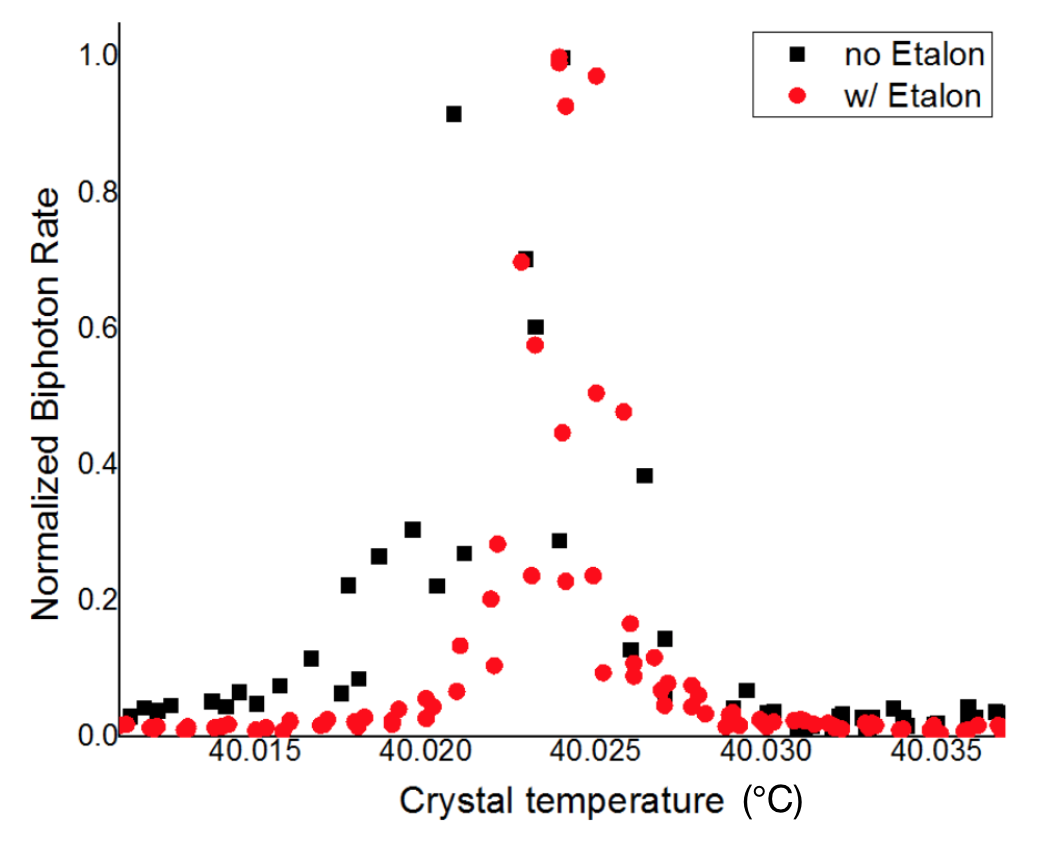
\includegraphics[width=0.4\linewidth]{no2_temp_etalon.png}}
    ~~~~
    \subcaptionbox
        {第三個模態
        \label{fig:subfig_fig2}}
        {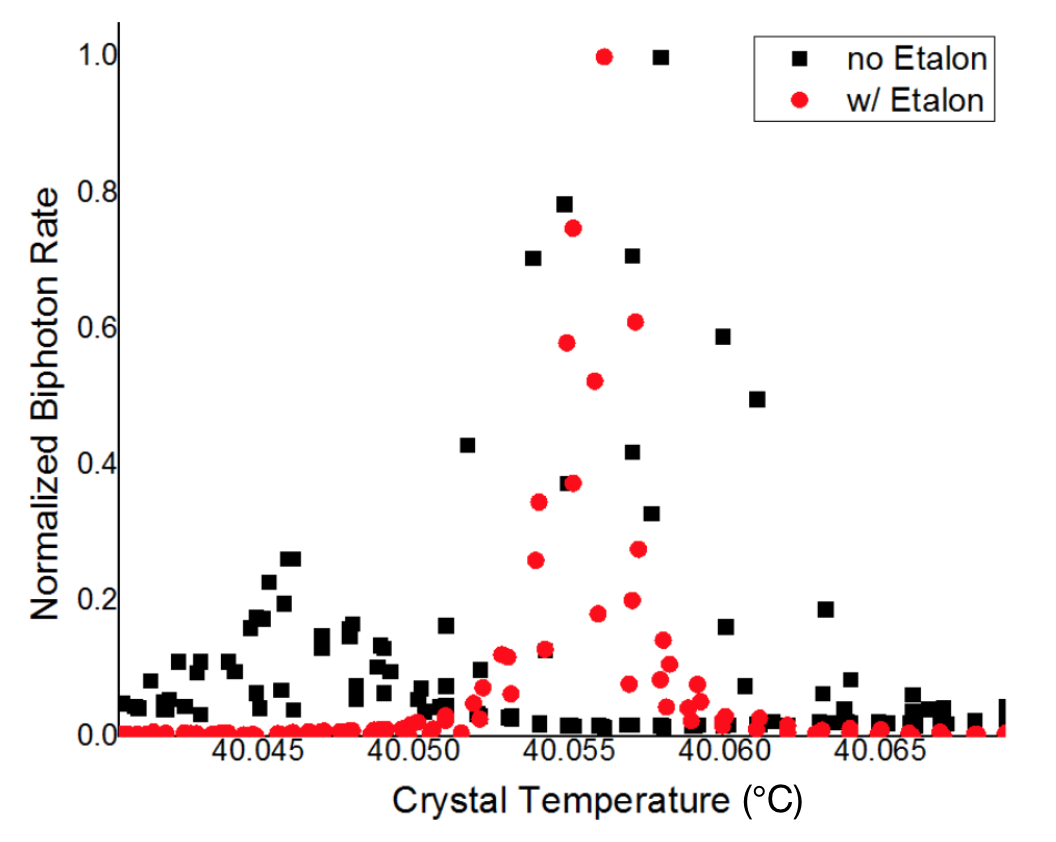
\includegraphics[width=0.4\linewidth]{no3_temp_etalon.png}}
    \caption[調整溫度測量雙光子產生率(加上濾波器)]{在沒放 $^{87}Rb$ 原子氣體管時之測量。黑色為無 Etalon 濾波器時測量之訊號,紅線為有加上 Etalon 濾波器測量到的訊號,兩者相比可看出,加上 Etalon 濾波器後測量到的頻寬較小,且明顯有部分的光被濾掉,可確定本來的光源為多模。}
    \label{fig:temp_scan_g2_with_etalon}
\end{figure}

\begin{figure}[!hbt]
    %\captionsetup[subfigure]{labelformat=empty} % 完全隱藏圖號
    \centering
    \subcaptionbox
        {第二個模態
        \label{fig:subfig_fig1}}
        {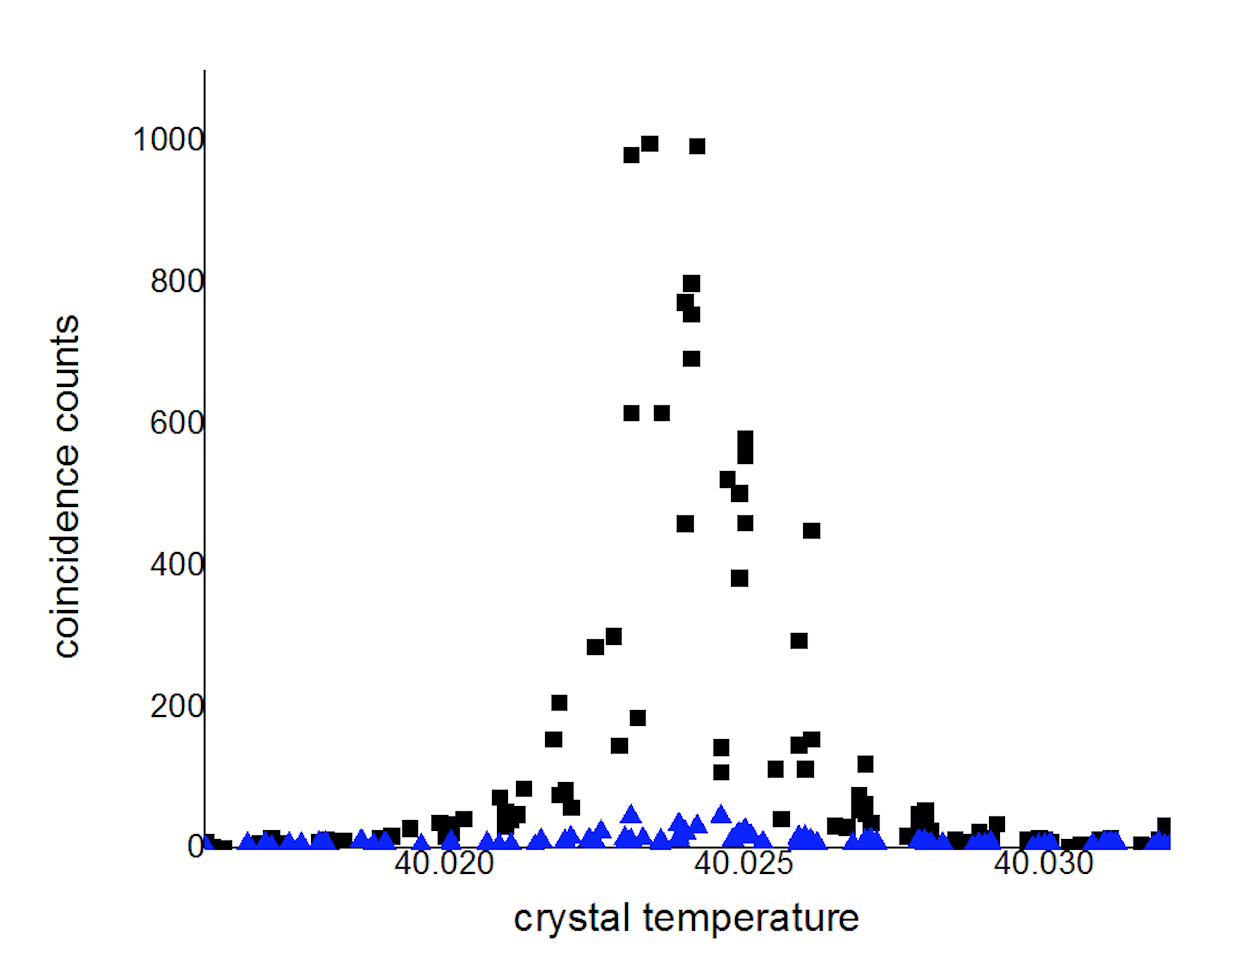
\includegraphics[width=0.4\linewidth]{second_mode_absorption.png}}
    ~~~~
    \subcaptionbox
        {第三個模態
        \label{fig:subfig_fig2}}
        {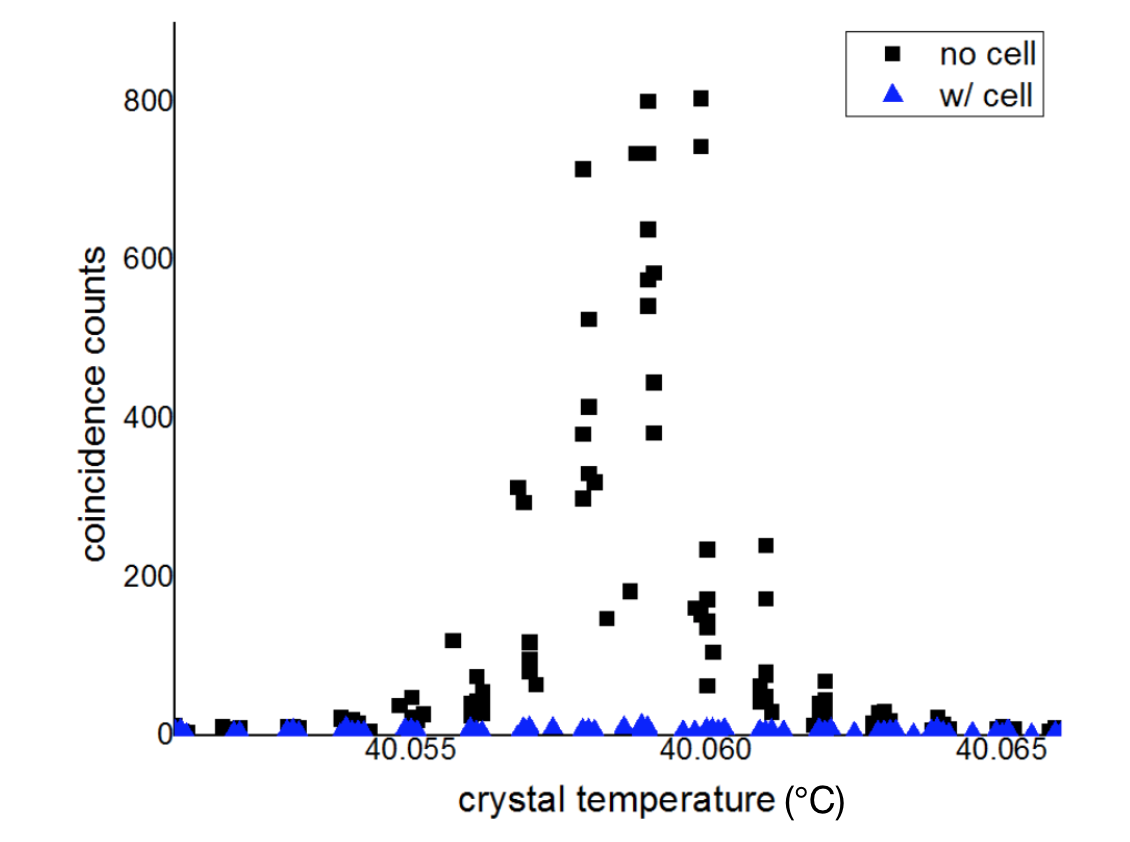
\includegraphics[width=0.4\linewidth]{third_mode_absorption.png}}
    \caption[加上 Etalon 濾波器之後,光就能完全被原子吸收]{加上 Etalon 濾波器之後,測量光子對原子之穿透率。黑色為未放 $^{87}Rb$ 原子時測量到的訊號,藍色為放了 $^{87}Rb$ 原子後測量到的訊號,光幾乎完全被  $^{87}Rb$ 吸收。}
    \label{fig:absorption_etalon_temp_scanning}
\end{figure}

\end{document}